% --------------------------------------------------------------------------------

\begin{exercise}

\phantom{}

\begin{enumerate}[label = \textbf{\alph*)}]
  \item Beweisen Sie die Aussage in Kapitel 1, Exercise 6 des Vorlesungsskriptes.
  \item Beweisen Sie die Aussage in Kapitel 1, Exercise 7 des Vorlesungsskriptes.
\end{enumerate}

\end{exercise}

% --------------------------------------------------------------------------------

\begin{solution}

\phantom{}

\begin{enumerate}[label = \textbf{\alph*)}]

  \item \phantom{}
  
  \begin{figure}[h!]
    \centering
    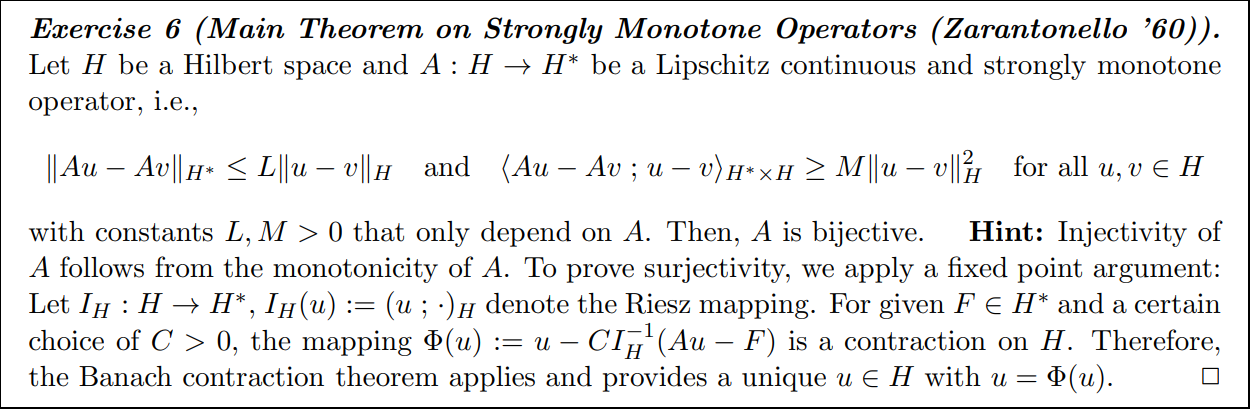
\includegraphics[width = 0.9 \textwidth]{Exercise 6.png}
  \end{figure}
  
  Wir zeigen zunächst die Injektivität. Gelte $Au = Av$, dann folgt

  \begin{align*}
    0 = \langle Au - Av; u - v \rangle_{H^*\times H}
    \geq M\|u -v\|_H^2
  \end{align*}

  und somit $u = v$. \\
  Zur Surjektivität definieren wir die bijektive Riesz-Abbildung

  \begin{align*}
    I_H: H \to H^*, \quad u \mapsto (u;\cdot)_H
  \end{align*}

  und für beliebig feste $F \in H^*, C > 0$

  \begin{align*}
    \Phi: H \to H, \quad u \mapsto u - CI_H^{-1}(Au - F).
  \end{align*}

  Wir berechnen mit $C < \frac{M}{L^2}$

  \begin{align*}
    \|\Phi(u) - \Phi(v)\|_H^2 &= (u - CI_H^{-1}(Au - F) -v + CI_H^{-1}(Av - F); u - CI_H^{-1}(Au - F) -v + CI_H^{-1}(Av - F)) \\
    &= (u  -v + CI_H^{-1}(Av - Au); u -v + CI_H^{-1}(Av - Au)) \\
    &= (u  - v; u - v) + (CI_H^{-1}(Av - Au); CI_H^{-1}(Av - Au)) + 2(u-v; CI_H^{-1}(Av - Au)) \\
    &\leq \|u - v\|_H^2 + C^2\|Av - Au\|_{H^*}^2 + 2C(I_H^{-1}(Av - Au); u-v) \\
    &\leq \|u - v\|_H^2 + C^2L^2\|u - v\|_{H}^2  - 2C I_H((I_H^{-1}(Av - Au))(v-u) \\
    &= \|u - v\|_H^2 + C^2L^2\|u - v\|_{H}^2 - 2C (Av - Au))(v-u) \\
    &\leq \|u - v\|_H^2 + C^2L^2\|u - v\|_{H}^2 - 2CM\|u-v\|_H^2\\
    &= \|u - v\|_H^2(1 + C^2L^2 - 2CM)\\
    &< \left(1 - \frac{M^2}{L^2}\right)\|u - v\|_H^2\\
  \end{align*}

  Damit existiert nach dem Banachschen Fixpunktsatz ein eindeutiges $u \in H$ mit

  \begin{align*}
    u = \Phi(u) = u - CI_H^{-1}(Au - F)
    \implies I_H^{-1}(Au - F) = 0 \implies Au = F.
  \end{align*}

  Da $F \in H^*$ beliebig war, ist damit auch die Surjektivität gezeigt.

  \item \phantom{}
  
  \begin{figure}[h!]
    \centering
    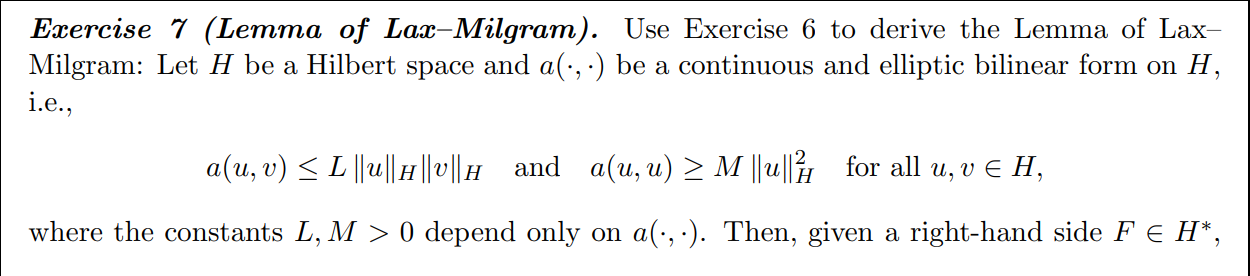
\includegraphics[width = 0.9 \textwidth]{Exercise 7.1.png}
    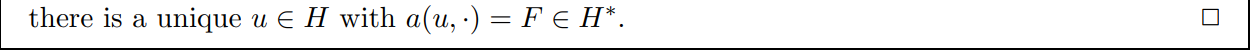
\includegraphics[width = 0.9 \textwidth]{Exercise 7.2.png}
  \end{figure}

  Definiere den Operator

  \begin{align*}
    A: H \to H^*, \quad u \mapsto a(u,\cdot).
  \end{align*}

  Aus den Voraussetzungen folgt

  \begin{align*}
    \forall w \in H: \|(A(u)- A(v))w\| = \|a(u,w) - a(v,w)\| = \|a(u - v,w)\| \leq L\|u-v\|_H\|w\|_H
  \end{align*}

  und damit $\|A(u) - A(v)\|_{H^*} \leq L\|u-v\|_H$.
  Weiters gilt:

  \begin{align*}
    \langle Au - Av; u - v \rangle_{H^*\times H} = (u - v; u - v) \geq M\|u-v\|_H^2
  \end{align*}

  Also können wir obigen Satz anwenden und erhalten zu jedem $F \in H^*$ ein eindeutiges $u \in H$ mit

  \begin{align*}
    a(u,\cdot) = F.
  \end{align*}

\end{enumerate}

\end{solution}

% --------------------------------------------------------------------------------
